%


\documentclass[twoside]{article}
\setlength{\oddsidemargin}{0.25 in}
\setlength{\evensidemargin}{-0.25 in}
\setlength{\topmargin}{-0.6 in}
\setlength{\textwidth}{6.5 in}
\setlength{\textheight}{8.5 in}
\setlength{\headsep}{0.75 in}
\setlength{\parindent}{0 in}
\setlength{\parskip}{0.1 in}

%
% ADD PACKAGES here:
%

\usepackage{amsmath,amsfonts,graphicx}

%
\newcounter{lecnum}
\renewcommand{\thepage}{\thelecnum-\arabic{page}}
\renewcommand{\thesection}{\thelecnum.\arabic{section}}
\renewcommand{\theequation}{\thelecnum.\arabic{equation}}
\renewcommand{\thefigure}{\thelecnum.\arabic{figure}}
\renewcommand{\thetable}{\thelecnum.\arabic{table}}

%
% The following macro is used to generate the header.
%
\newcommand{\lecture}[4]{
   \pagestyle{myheadings}
   \thispagestyle{plain}
   \newpage
   \setcounter{lecnum}{#1}
   \setcounter{page}{1}
   \noindent
   \begin{center}
   \framebox{
      \vbox{\vspace{2mm}
    \hbox to 6.28in { {\bf EE302 - Feedback Systems
	\hfill Spring 2019} }
       \vspace{4mm}
       \hbox to 6.28in { {\Large \hfill Lecture #1 \hfill} }
       \vspace{2mm}
       \hbox to 6.28in { {\it Lecturer: #2 \hfill } }
      \vspace{2mm}}
   }
   \end{center}
   \markboth{Lecture #1}{Lecture #1}

   \vspace*{4mm}
}

%Use this command for a figure; it puts a figure in wherever you want it.
%usage: \fig{NUMBER}{SPACE-IN-INCHES}{CAPTION}
\newcommand{\fig}[3]{
			\vspace{#2}
			\begin{center}
			Figure \thelecnum.#1:~#3
			\end{center}
	}
% Use these for theorems, lemmas, proofs, etc.
\newtheorem{theorem}{Theorem}[lecnum]
\newtheorem{lemma}[theorem]{Lemma}
\newtheorem{proposition}[theorem]{Proposition}
\newtheorem{claim}[theorem]{Claim}
\newtheorem{corollary}[theorem]{Corollary}
\newtheorem{definition}[theorem]{Definition}
\newenvironment{proof}{{\bf Proof:}}{\hfill\rule{2mm}{2mm}}

% **** IF YOU WANT TO DEFINE ADDITIONAL MACROS FOR YOURSELF, PUT THEM HERE:

\begin{document}

% Lecture Details
\lecture{19}{Asst. Prof. M. Mert Ankarali}

\par

\section{Lead Compensator Design}

The lead-compensator is a controller which has the form of a
first-order high-pass filter 
%
\begin{align*}
  G_{c}(s) = K_{c} \frac{T s + 1}{T \alpha s + 1}
  \quad \alpha \in (0,1)
\end{align*}
%
In general, we first design $K_{c}$ based on the setady-state
requirements of the system, and then design $T$ and $\alpha$
based on the phase-margin requirement.  First let's illustrate the bode-plots of a unity gain lead-compensator
to understand how we can utilize its properties for the 
design process. 

     \begin{center}
 \begin{minipage}[h]{\linewidth}
     \begin{center}
       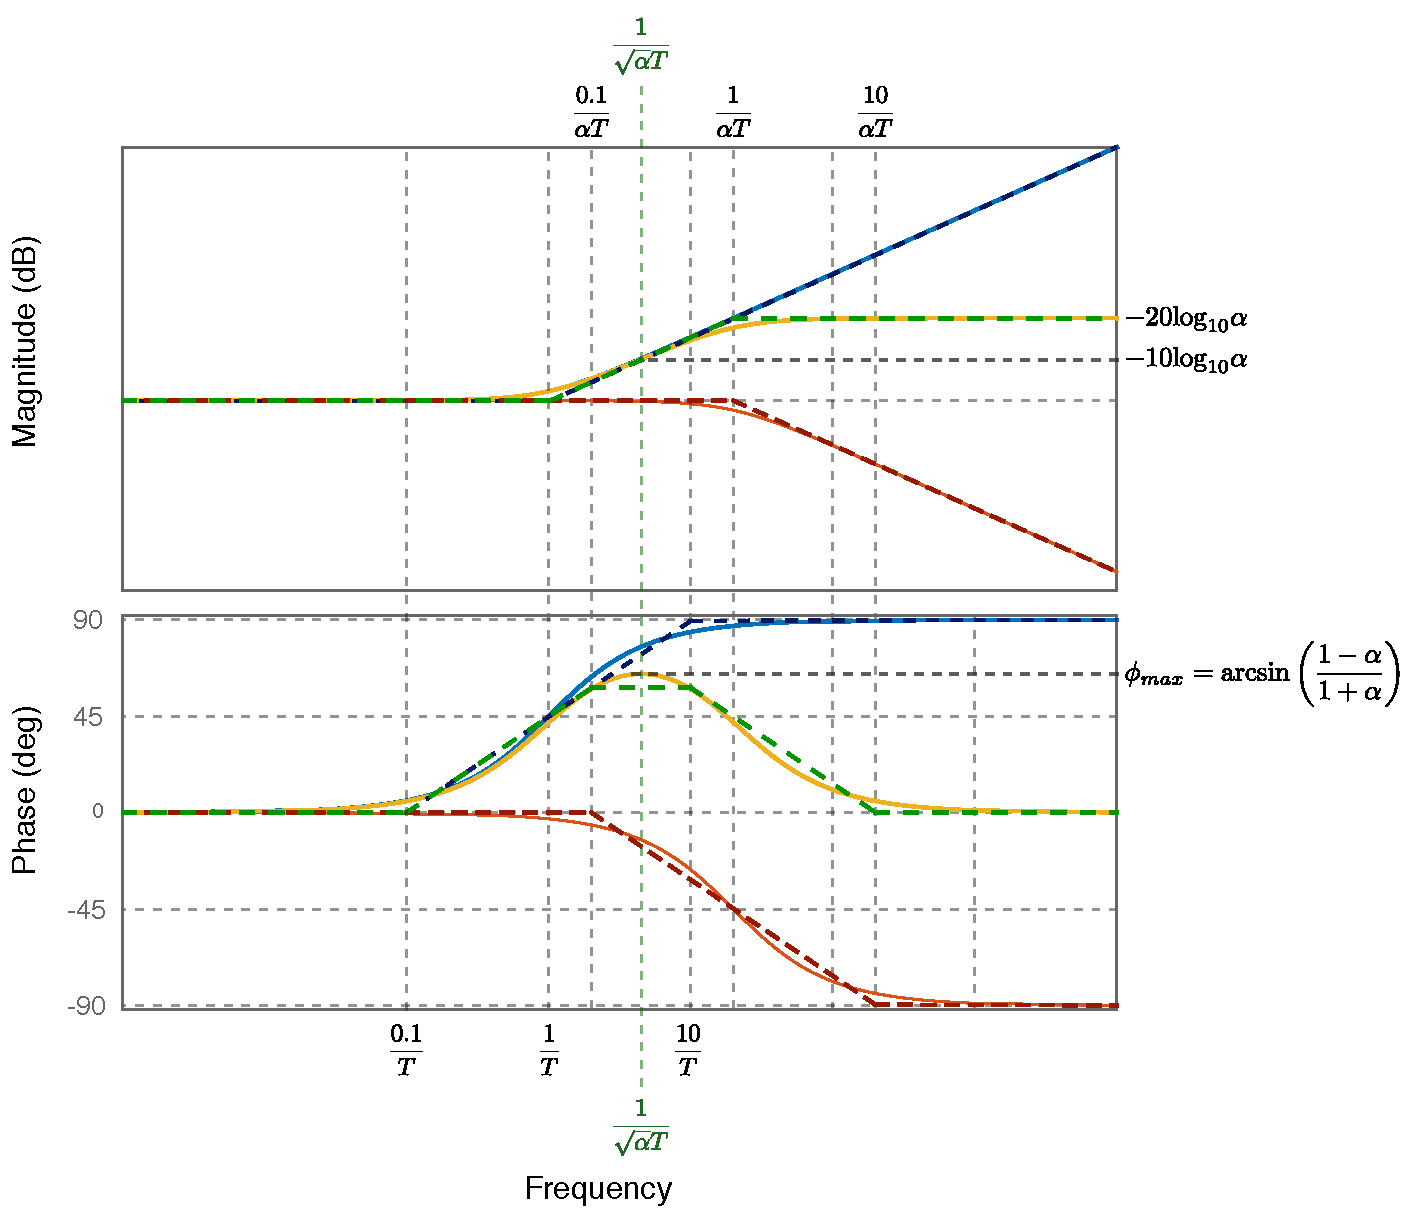
\includegraphics[width=0.9\textwidth]{leadnew}
     \end{center}
 \end{minipage}
     \end{center}

We can see that (both from the actual and approximate bode-plots),
phase-lead compensator is a type of high-pass filter for which 
the cut-off (mid) frequency is $\omega_c = \frac{1}{\sqrt{\alpha} T}$.
The low and high frequency gains are respectively $0$ dB and $-20
\mathrm{log}_{10} \alpha$ dB. The lead-compensator phase,
$\phi_{max}$, peaks at its cut-off frequency, and basically we will
try to use this positive maximum phase shift to improve the phase 
margin of the feedback 
system.

Let's derive a formula for $\phi_{max}$, which we will need during the 
design phase
%
\begin{align*}
    \phi_{max} &= \angle [ G_c( j \omega_c) ] = \angle \left[ 1 + T
  \omega_c j \right] - \angle \left[ 1 + \alpha T
  \omega_c j \right] = \arctan(T \omega_c) - \arctan(\alpha  T \omega_c)
  \\
  &= \arctan \left( \frac{1}{\sqrt{\alpha}}  \right) - \arctan \left(
    \sqrt{\alpha} \right) 
    \\
  &= \pi/2 - 2 \arctan \left( \sqrt{\alpha} \right)
\\
\sin \phi_{max} &=  \cos \left( 2 \arctan \left( \sqrt{\alpha} \right)
                  \right)
                  = 1 - 2 \left[ \sin\left( \arctan \left( \sqrt{\alpha} \right)
                  \right) \right]^2 = 1 - 2 \frac{\alpha}{1 + \alpha}
                  \\
&= \frac{1 - \alpha}{1 + \alpha}
  \\
    \phi_{max} &= \arcsin \left( \frac{1 - \alpha}{1 + \alpha} \right)
        \         \Rightarrow \ \alpha = \frac{1 - \sin \phi_{max}}{1
                 + \sin \phi_{max}}
\end{align*}
%
As expected when $\alpha = 1$, $\phi_{max} = 0$ since numerator 
and denominator time constants becomes equal in this
case. Accordingly, we can see that 
%
\begin{align*}
  \alpha \searrow \ \Rightarrow \ \phi_{max} \nearrow
\end{align*}
%
Theoretical maximum value for $\phi_{max}$ is $90^o$,
however practically $\phi_{max} < 75^o$ for analog 
lead compensator circuits. Another important factor that 
we will need to pay attention is the gain-shift of
the lead-compensator at the cut-off frequency 
%
\begin{align*}
  M_{dB}(j \omega_c) = -10 \mathrm{log}_{10} \alpha \quad \& \quad
  | G(j \omega_c) | = \frac{1}{\sqrt{\alpha}}
\end{align*}
%

We will illustrate the design process on an example 

\vspace{6pt}

\textbf{Ex:} Consider the following feedback system illustrated below.
It is given that $G(s) = \frac{1}{s (s+1)}$ and we want to
design a lead-compensator, $G_c(s) = K_c \frac{T s + 1}{T \alpha s +
  1}$, such that unit-ramp steady-state error satisfies, $e_{ss} = 0.1$ and phase-margin of the compensated system satisfies $\phi_m^* =
\left[ 45^0 , 55^0 \right]$. 

\vspace{6pt}

     \begin{center}
 \begin{minipage}[h]{\linewidth}
     \begin{center}
       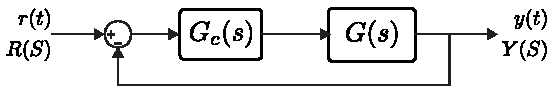
\includegraphics[width=0.6\textwidth]{ex1block}
     \end{center}
 \end{minipage}
     \end{center}

\vspace{6pt}

\textbf{Solution:}

\textbf{Step 1:} We design/compute $K_c$ based on the steady-state 
requirement on the unit-ramp error.  
%
\begin{align}
   e_{ss} = \frac{1}{K_v} = \frac{1}{K_c} = 0.1 \ \rightarrow \ K_c = 10
\end{align}

\textbf{Step 2:} Embed $K_c$ into $G(s)$, i.e. 
%
\begin{align*}
  \bar{G}(s) = K_c G(s) = \frac{10}{s (s+1)} ,
\end{align*} 
%
draw the bode-plot for $\bar{G}(s)$, and compute the gain-crossover
frequency, $\omega_{gc}$, and the phase margin, $\phi_M$, for the
uncompensated $\bar{G}(s)$. The bode plot of $\bar{G}(s)$ and its
approximation is illustrated in the Figure below. 

     \begin{center}
 \begin{minipage}[h]{\linewidth}
     \begin{center}
       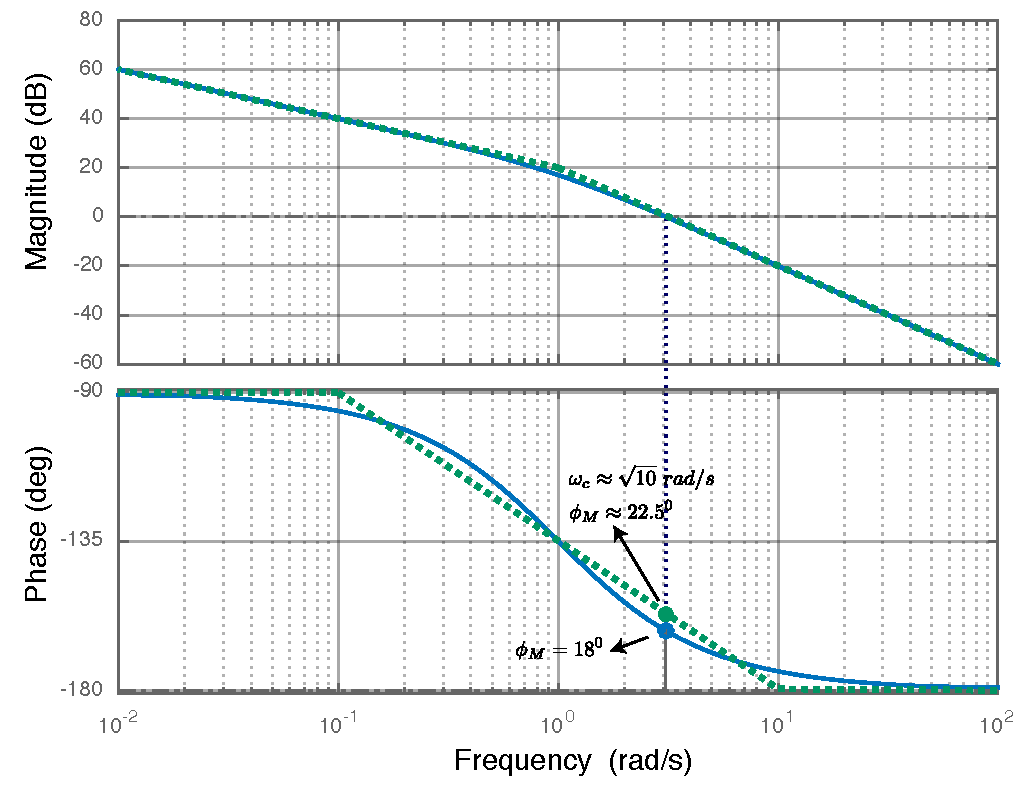
\includegraphics[width=0.85\textwidth]{bodesystem}
     \end{center}
 \end{minipage}
     \end{center}

If we concentrate on the approximate bode-plots, we can estimate
the gain-crossover frequency and the phase-margin as
%
\begin{align*}
  \omega_{gc} &\approx \sqrt{10} \ rad/s = 3.16 \ rad/s
  \\
  \phi_m &\approx 22.5^o
\end{align*}
%
If we compute the actual values from the actual Bode plot, we obtain
%
\begin{align*}
  \omega_{gc} &= 3.08 \ rad/s
  \\
  \phi_m &\approx 18^o
\end{align*}
%
We can see that approximation is pretty good for the
$\omega_c$, however a little crude for $\phi_m$. 
So let's compute $\angle [ G(j \omega_{gc}) ] $ for 
$\omega_{gc} \approx \sqrt{10}$ and estimate the 
phase-margin based on this frequency
%
\begin{align*}
  \angle [ G(j \omega_{gc}) ] &= \angle [ G(j \sqrt{10}) ] =
 -90^0 - \arctan \left( \sqrt{10} \right) =  -162.5^o
  \\
 \phi_M \approx 17.5^o
\end{align*}

\textbf{Step 3:} Compute the required phase increment, $\Delta \phi$ to be
added by the compensator and compute $\alpha$
%
\begin{align*}
   \phi_{max} &\approx \Delta \phi = \phi_M^* - \phi_M + \epsilon
  \\
  \epsilon &= 5^0 - 10^0
\end{align*}
%
So for the given problem, we can compute $\phi_{max}$
and $\alpha$ as
%
\begin{align*}
   \phi_{max} &\approx 47.5^o - 17.5^0 + 7^0 = 37^0
                \\
  \alpha &= \frac{1 - \sin \phi_{max}}{1 + \sin \phi_{max}} \approx \frac{1}{4}
\end{align*}

\textbf{Step 4:} Estimate the ``new'' gain-crossover frequency, 
$\hat{\omega}_{gc}$, and place the peak point of the lead-compensator,
at this estimated $\hat{\omega}_{gc}$. 

We already know that, lead-compensator at its
center/cutoff frequency shifts the bode magnitude 
by $-10 \mathrm{log}_{10} \alpha$ (or increases the gain 
by $\frac{1}{\sqrt{6}}$) and this causes a shift in
gain-crossover frequency. 
For this reason, we can estimate the new gain-crossover
frequency as the point where the bode magnitude of 
$\bar{G}(s)$ crosses $10 \ \mathrm{log}_{10} \alpha$,
i.e. 
%
\begin{align*}
  M_{dB}( j \hat{\omega}_{gc} ) = 10 \ \mathrm{log}_{10} \alpha
\quad or \quad
  |G(j \hat{\omega}_{gc})| = \sqrt{\alpha}
\end{align*}
%
In our problem, 
%
\begin{align*}
  M_{dB}( j \hat{\omega}_{gc} ) \approx -6 \ dB
\quad or \quad
  |G(j \hat{\omega}_{gc})| = \frac{1}{2}
\end{align*}
%
We can indeed estimate the new gain-crossover frequency graphically from the
bode-plot. The figure below, illustrates how we can find 
the new-gain crossover frequency graphically

     \begin{center}
 \begin{minipage}[h]{\linewidth}
     \begin{center}
       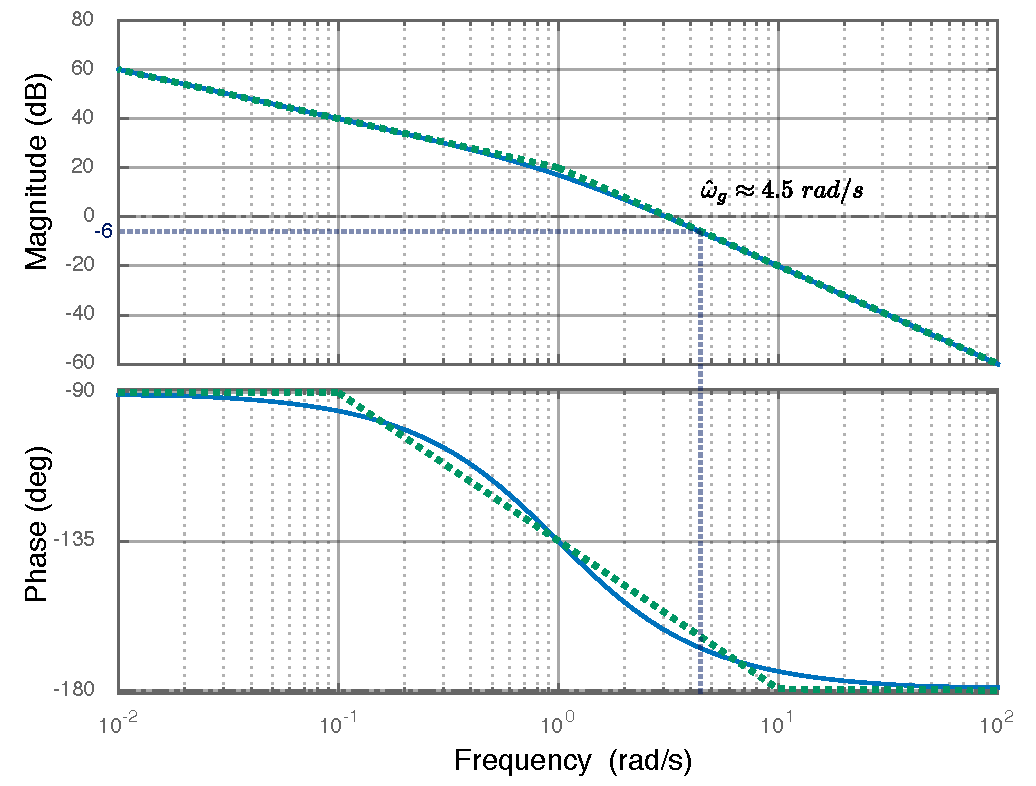
\includegraphics[width=0.85\textwidth]{gaincros}
     \end{center}
 \end{minipage}
     \end{center}

where $\hat{\omega}_{gc} \approx 4.5 \ rad/s$.
We can also estimate the new-gain crossover frequency
numerically 
%
\begin{align*}
  |G(j \hat{\omega}_{gc})| = \frac{1}{2}
  \\
  \frac{100}{\hat{\omega}_{gc}^2 \left( \hat{\omega}_{gc}^2 + 1
  \right)} = \frac{1}{4}
  \\
  \hat{\omega}_{gc}^4 + \hat{\omega}_{gc}^2 - 400 = 0
  \\
   \hat{\omega}_{gc} \approx 400^{1/4} = 4.47 \ rad/s
\end{align*}
%
which is very close to the graphical estimation. 

\textbf{Step 5:} Compute $T$ using $\hat{\omega}_{gc}$ and 
check if the lead-compensator meets the phase-margin
requirement. Otherwise, repeat the process with a higher
$\Delta \phi$ angle.
%
\begin{align*}
  \hat{\omega}_{gc} = \omega_c = \frac{1}{\sqrt{\alpha} T}
                      \quad \Rightarrow \quad 
  T = \frac{1}{\sqrt{\alpha} \hat{\omega}_{gc}}
\end{align*}
%
In our example 
%
\begin{align*}
     T = \frac{1}{\frac{4.5}{2}} \approx 0.45
         \quad \Rightarrow \quad
   G_c(s) = 10 \frac{0.45 s + 1}{0.1125 s + 1} = 40 \frac{s + 2.25}{s + 9}
\end{align*}
%
The Figure below illustrates the bode plots of both 
compensated and uncompensated ($\bar{G}(s) = K_c G(s)$) systems.
Compensated systems has a phase margin of $\phi_m = 49.7^o$
which meets the requirements.
%
     \begin{center}
 \begin{minipage}[h]{\linewidth}
     \begin{center}
       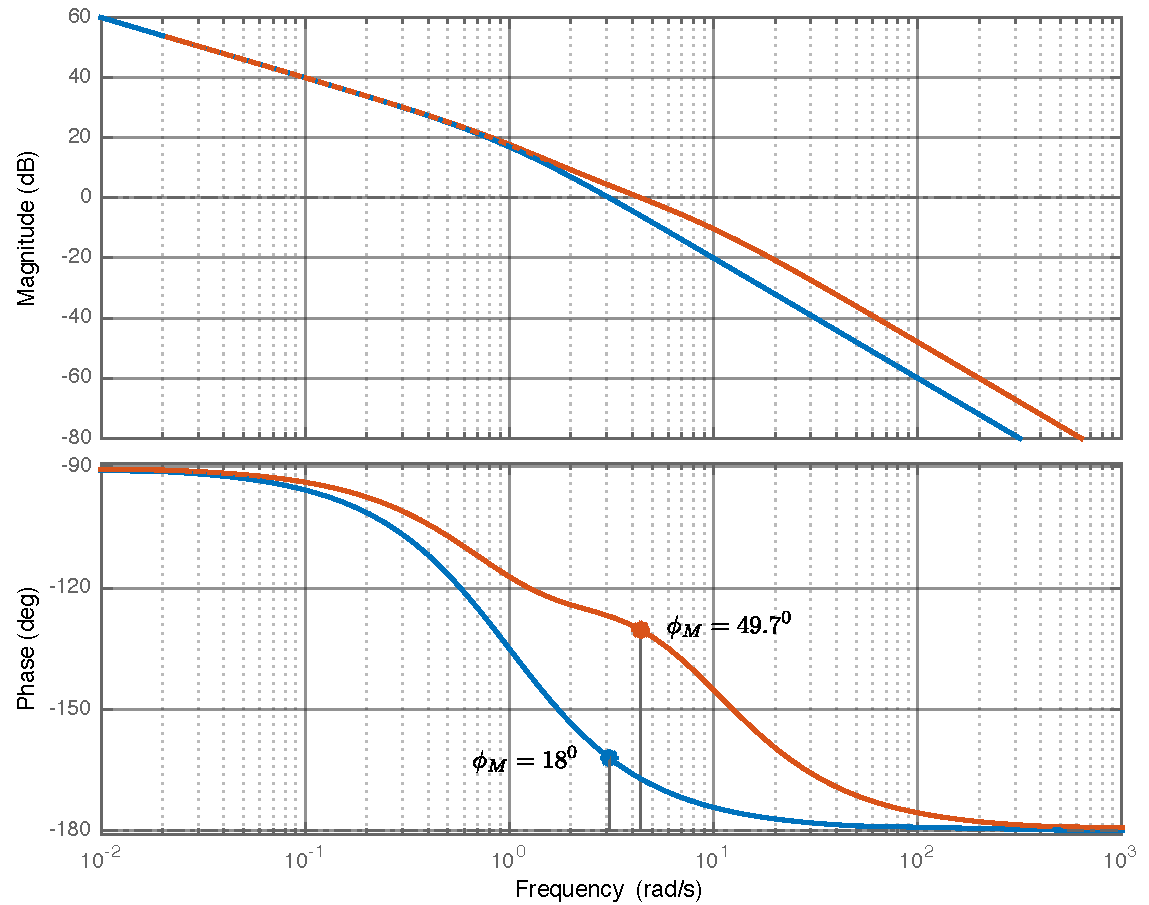
\includegraphics[width=0.85\textwidth]{comparison}
     \end{center}
 \end{minipage}
     \end{center}
%
Now let's compute new phase margin directly using the 
new gain-crossover frequency  
%
\begin{align*}
	\phi_{M} &= -180^o + \angle [ G_c(j 4.45 \ rad/s) \bar{G}( j 4.45 \ rad/s) ]
		= -180^o + 37^o + \angle [ \bar{G} ( j 4.45 \ rad/s) ]
		\\
		&= -180^o + 37^o - 90^o - \angle [ j 4.45 + 1 ]	
	= -180^o + 37^o - 90^o - 77^0
		\\
		&= 50^o 
\end{align*}
%
which is consistent with the phase-margin on the bode-plot.
In Figure below, we compare the closed-loop step responses
of both uncompensated and compensated closed-loop
transfer functions. We can clearly see that, the lead-compensator
substantially improves both the settling time 
and over-shoot performance. 

     \begin{center}
 \begin{minipage}[h]{0.7\linewidth}
     \begin{center}
       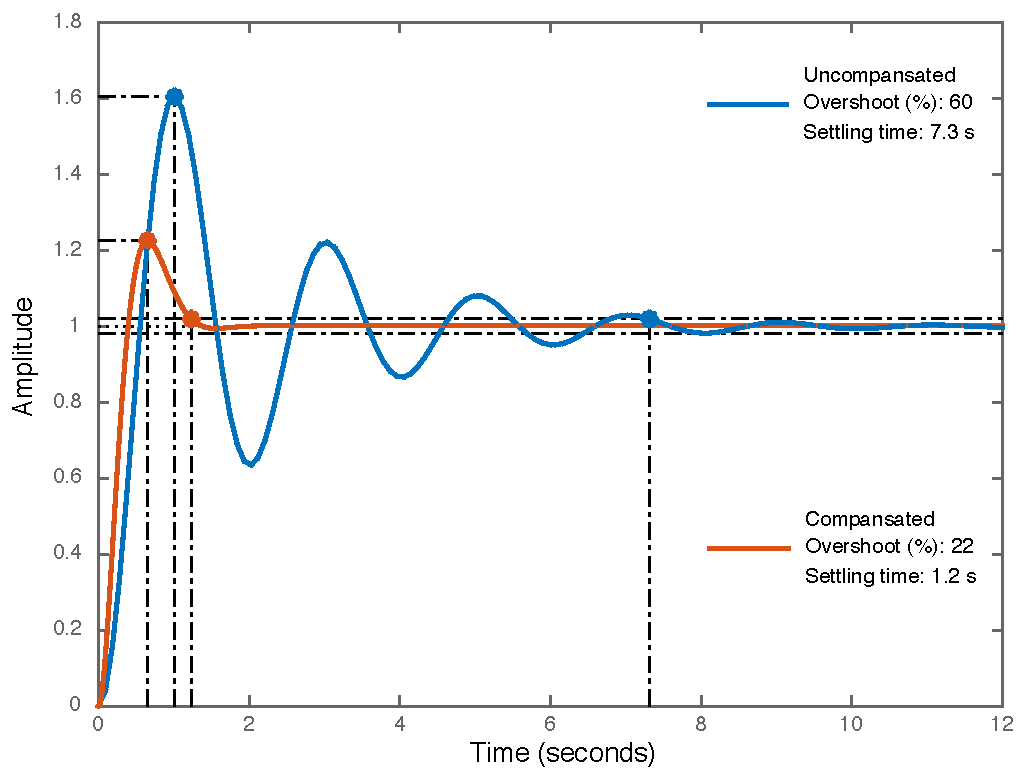
\includegraphics[width=\textwidth]{step}
     \end{center}
 \end{minipage}
     \end{center}

\paragraph{Phase-Lead Design Guideline:} 
\begin{enumerate}
	\item Design/compute $K_c$ based on the steady-state requirements 
	%
	\item Embed $K_c$ into $G(s)$, i.e. $ \bar{G(s)} = K_c G(s)$, then 
	draw the bode-plots for $\bar{G}(s)$, and compute the gain-crossover
	frequency, $\omega_{gc}$, and the phase margin, $\phi_M$, for the
	uncompensated $\bar{G}(s)$. 
	%
	\item Compute the required phase increment, $\Delta \phi$ to be
	added by the compensator and design/compute $\alpha$
	\item Estimate the ``new'' gain-crossover frequency, 
	$\hat{\omega}_{gc}$, and place the peak point of the lead-compensator,
	at this estimated $\hat{\omega}_{gc}$. 
	\item Check the phase-margin if it does not meet the requirements
	increase $\Delta \phi$ and repeat the process. 
\end{enumerate}

\newpage

\section{Lag Compensator Design}

The lag-compensator is a controller which has the form of a
first-order low-pass filter 
%
\begin{align*}
  G_{c}(s) = K_{c} \frac{T s + 1}{T \alpha s + 1}
  \quad \alpha \in (1,\infty)
\end{align*}
%
In general, we first design $K_{c}$ based on the steady-state
requirements of the system, then design $\alpha$
based on the phase-margin requirement, and finally 
choose a $T$ such that phase-lag of the compensator
does not interfere with the gain-crossover frequency.

First let's illustrate the bode-plots of a unity gain lag-compensator
to understand how we can utilize its properties for the 
design process. 

     \begin{center}
 \begin{minipage}[h]{\linewidth}
     \begin{center}
       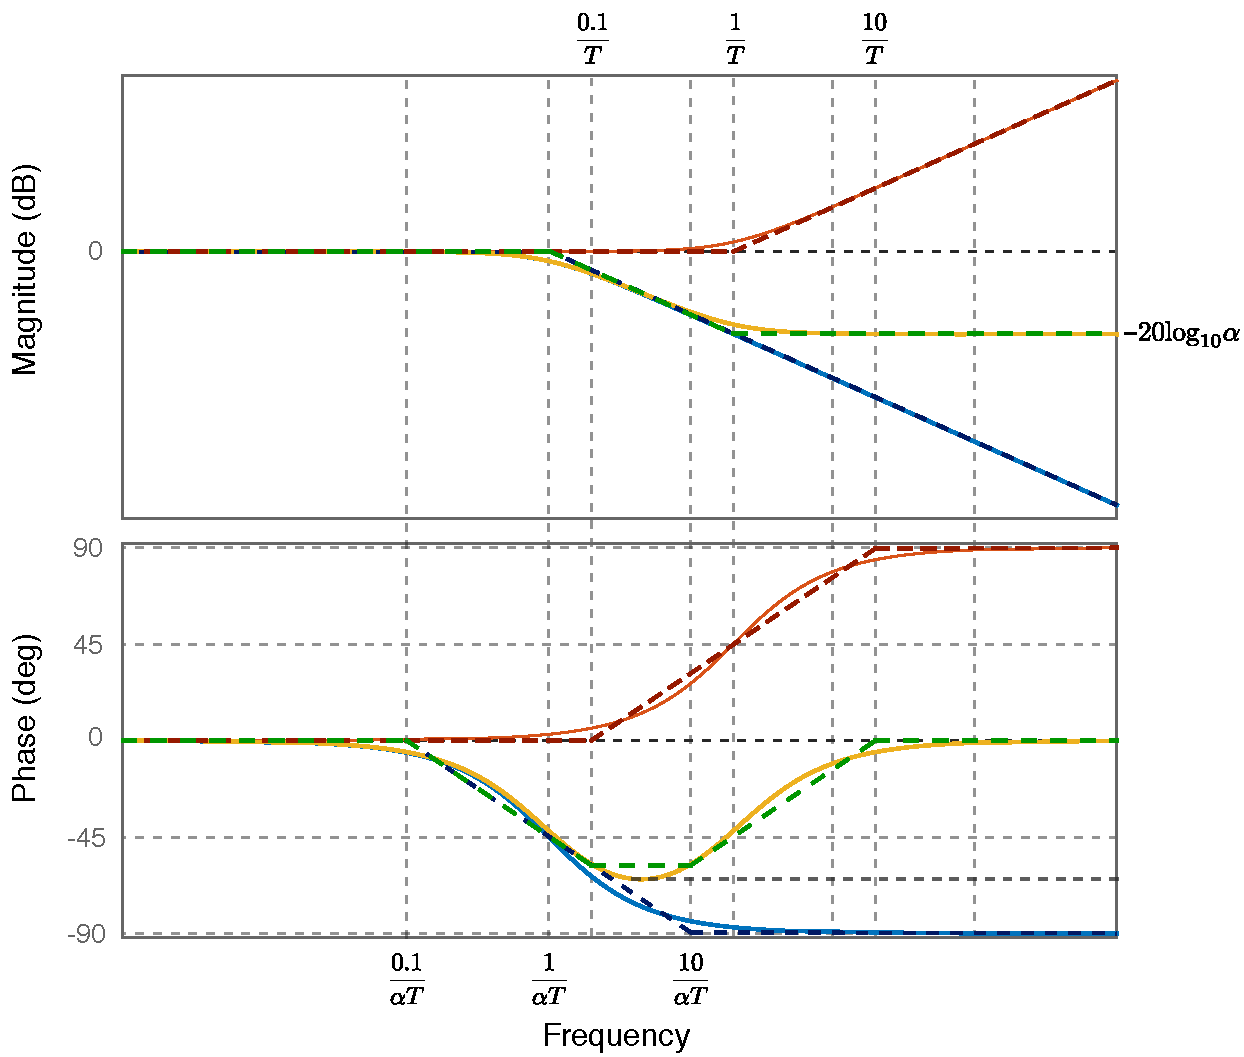
\includegraphics[width=0.8\textwidth]{lag}
     \end{center}
 \end{minipage}
     \end{center}

In lag-compensator design, we basically use the negative-gain shift of
the compensator in the high-frequency region and we try to push the
low and mid frequency region to the left (in frequency axis) such that 
they don't interfere with the gain-crossover frequency. For this
reason, design process easier compared to the lead-compensator. 

We will illustrate the lag-compensator design process on an the same example 

\vspace{6pt}

\textbf{Ex:} Consider the feedback system that we analyzed
previously in lead compensatory case. Plant is same, 
$G(s) = \frac{1}{s (s+1)}$. However now we want to
design a lag-compensator, $G_c(s) = K_c \frac{T s + 1}{T \alpha s + 1}
, \ a \in (1,\infty))$, such that unit-ramp steady-state error satisfies, $e_{ss}
0.1$ and phase-margin of the compensated system satisfies $\phi_m^*
> 40^o$. 

\textbf{Solution:}

\textbf{Step 1:} Same as the lead-design, we design/compute $K_c$ based on the steady-state 
requirement on the unit-ramp error.  
%
\begin{align}
   e_{ss} = \frac{1}{K_v} = \frac{1}{K_c} = 1 \ \rightarrow \ K_c = 10
\end{align}

\textbf{Step 2:} Embed $K_c$ into $G(s)$, i.e. 
%
\begin{align*}
  \bar{G(s)} = K_c G(s) = \frac{10}{s (s+1)} ,
\end{align*} 
%
draw the bode-plot for $\bar{G}(s)$. 

\textbf{Step 3:} Compute/find the required gain-crossover
frequency, $\omega_{gc}^*$, based on
the required phase-margin, $\phi^*_M$, and compute/find 
the magnitude of $G(s)$ at $\omega_{gc}^*$, i.e. 
$| \bar{G}(j  \omega_{gc}^*) | $ or $20 \mathrm{log}_20 | \bar{G}(j  \omega_{gc}^*) |$.
%
\begin{align*}
  \angle [ \bar{G}(j  \omega_{gc}^*) ] &= -180^o + \phi_M^* + \epsilon
  \\
  \epsilon &\approx 5^0
\end{align*}
%
Note that at high-frequency 
region, lag-compensator acts like negative gain 
shift on magnitude plot while not affecting the 
phase response. Such a gain shift technically 
changes the gain-crossover frequency, which
can be potentially used for changing the phase 
margin. 

For our example, compensated gain-crossover frequency can be computed as
%
\begin{align*}
  \angle [ \bar{G}(j  \omega_{gc}^*) ] = -135^o
  \quad \Rightarrow \quad \omega_{gc}^* \approx 1 \ rad/s
\end{align*}
%
The bode plot of $\bar{G(s)}$,
required gain-crossover frequency, and  
the magnitude of $\bar{G(s)}$ at the desired 
gain-crossover frequency are 
illustrated in the Figure below. 

     \begin{center}
 \begin{minipage}[h]{\linewidth}
     \begin{center}
       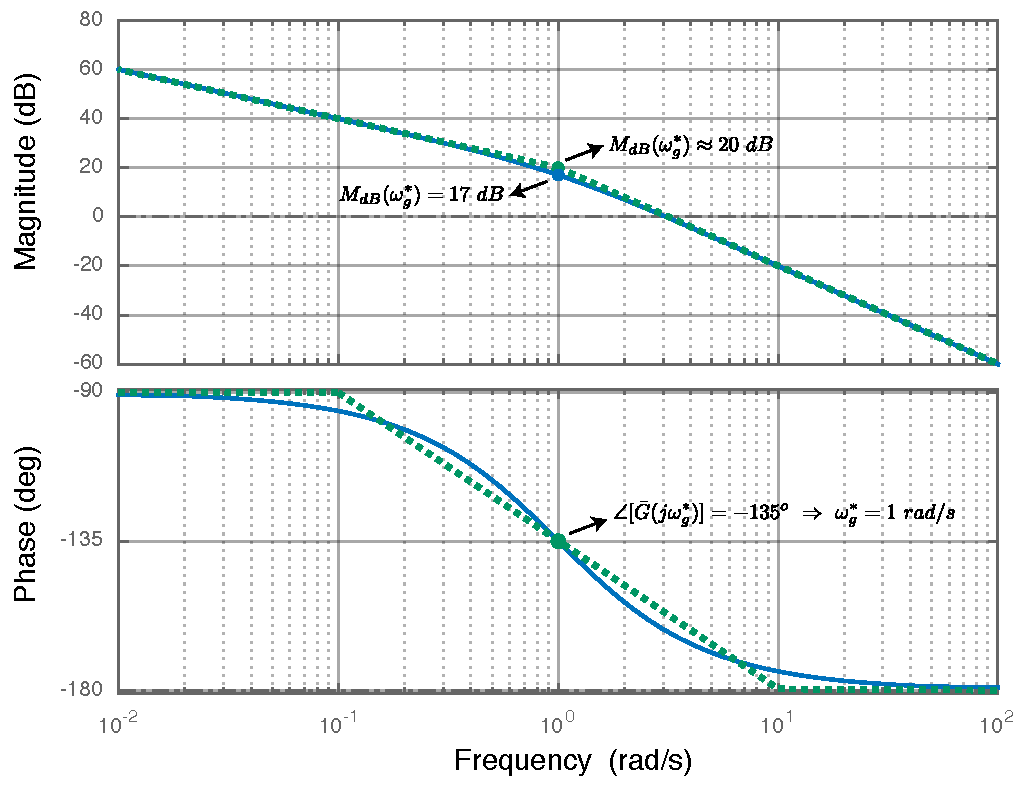
\includegraphics[width=0.8\textwidth]{laggaincross}
     \end{center}
 \end{minipage}
     \end{center}
     
From the bode-plots we can observe that 
at the desired  $\omega_{gc}^* \approx 1 \ rad/s$,
bode-plot approximation has a magnitude of
$20 \ dB$, whereas the magnitude in the actual
bode plot is approximately $17 \ dB$. In this example,
let's use the magnitude of the approximation in the
next Step.

\textbf{Step 4:} Compute $\alpha$ to compensate the 
the magnitude at the new-gain crossover frequency
%
\begin{align*} 
  20 log_{10} \alpha =  20 \mathrm{log}_{10} |\bar{G}(j  \omega_{gc}^*) |
  	\quad \mathrm{or} \quad
     \alpha = | \bar{G}(j  \omega_{gc}^*) |
\end{align*}
%
In our example, $\alpha$, can be computed as
%
\begin{align*} 
	20 log_{10} \alpha \approx 20 \ dB
	\ \Rightarrow \ \alpha \approx 10
\end{align*}
%

\textbf{Step 4:} Choose $T$ such that ``$10/T \leq \omega_{gc}^*$''.
Note that $10/T$ is the frequency where the phase of the compensator
approximately re-approaches to zero.
This is required in order the
          negative phase bump of the compensator does not affect the
          phase-margin. 
%
\begin{align*} 
	\frac{1}{T} \approx 0.1 \omega_{gc}^*
		\ \Rightarrow \ T \approx 10
		\\	
G_c(s) = 10 \frac{10 s + 1}{100 s + 1} = \frac{s + 0.1}{s + 0.01}
\end{align*}
%
The Figure below illustrates the bode plots of 
the uncompensated ($\bar{G}(s) = K_c G(s)$) system,
designed lag-compensator, and the compensated system. 
Compensated systems has a phase margin of $\phi_m = 45^o$
which meets the requirements.

     \begin{center}
 \begin{minipage}[h]{\linewidth}
     \begin{center}
       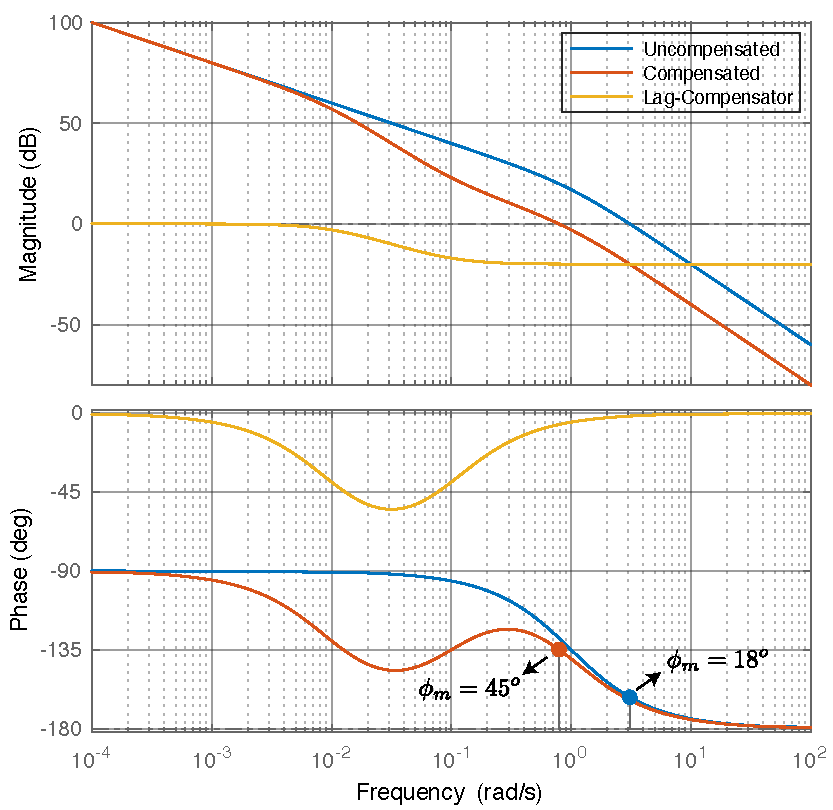
\includegraphics[width=0.75\textwidth]{complag}
     \end{center}
 \end{minipage}
     \end{center}

In Figure below, we compare the closed-loop step responses
of both uncompensated and compensated closed-loop
transfer functions. We can see that, similar to the the lead-compensator,
lag-compensator improves the over-shoot performance. 
However, the settling-time of the compensated system is approximately
two times of the original system. This is major the drawback of the lag-compensator. 

     \begin{center}
 \begin{minipage}[h]{0.65\linewidth}
     \begin{center}
       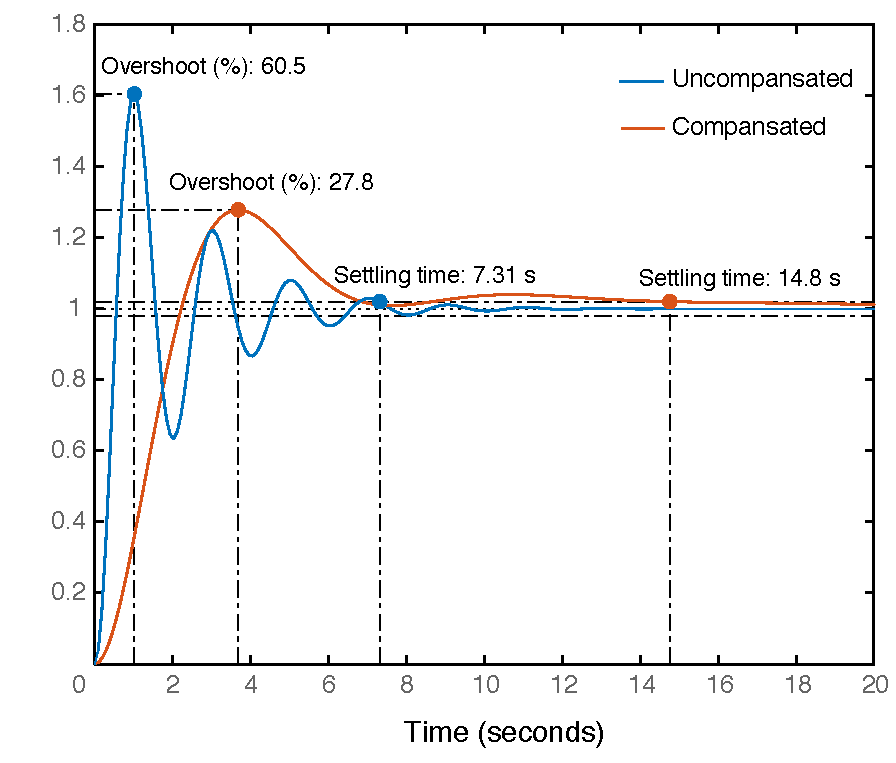
\includegraphics[width=\textwidth]{lagstep}
     \end{center}
 \end{minipage}
     \end{center}

The reason behind the reduced convergence speed performance is that
new gain-crossover frequency is less than the original gain-crossover frequency.
PM is closely related with over-shoot performance. On the other hand
gain-crossover frequency determines the band-with of the system 
which is closely related with the rise and settling times. 

\paragraph{Phase-Lag Design Guideline:} 
\begin{enumerate}
	\item Design/compute $K_c$ based on the steady-state requirements 
	%
	\item Compute/find the required gain-crossover
	frequency, $\omega_{gc}^*$, based on
	the required phase-margin, $\phi^*_M$, and compute/find 
	the magnitude of $G(s)$ at $\omega_{gc}^*$
	%
	\item Compute $\alpha$ to compensate the 
	the magnitude at the new-gain crossover frequency
	%
	\item Chose $T$ at such that ``$10/T \leq \omega_{gc}^*$''. This is required in order the
          negative phase bump of the compensator does not affect the
          phase-margin. Note that $10/T$ is the frequency where the phase of the compensator
          approximately re-approaches to zero.
	%
	\item Check the phase-margin if it does not meet the requirements
	change $\Delta \phi$ and repeat the process. 
\end{enumerate}


% **** This ENDS THE EXAMPLES. DON'T DELETE THE FOLLOWING LINE:
\end{document}